As it has be been shown in section \ref{sec:StateOfTheArt}, the current technique that exist nowadays cannot be used for tritium monitoring in quasi-real time since they have either higher LDL than the limit established by Council Directive, $100~\becquerel/\liter$, or they are a off-line method (too slow). 

As a result of these limitations appear the \textit{Tritium} project \cite{TRITIUM}, with the title of "Design, construction and commissioning of automatic stations for quasi-real time monitoring of low radioactive levels of tritium in water".

This project has been funded by Interreg Sudoe program of the European Economical Community, EEC, in the 2016 call with the reference number SOE1/P4/EO214. The purpose of this project is the development of a tritium monitor in quasi-real time. This monitor consists of a ultrapure water system, which prepare the sample before introducing it in our detector, the tritium detector, where the tritium measure will be done, the cosmic veto and the pasive shielding, which reduce the natural background of our tritium detector, and several types of electronic which control all these parts of the monitor, analyze the tritium measurement and will send an alarm if the configured limit ($100~\becquerel/\liter$) is overcome.

The difficulty when the measurement of tritium is done is to distinguish these signals from the background. This is because tritium signals are small since tritium events has low energy ($\sim~\keV$) and this is the energy range in the spectrum where there are more background counts (the lower energy in the spectrum, the more electronic noise). To reduce the background counts of TRITIUM monitor, coincidence techniques will be used.

%It is important to check the water tightness of each prototype because if the water reaches the photosensor it will be irreparably damaged. On top of that if we use high concentrations of tritium in water for laboratory tests we can contaminate this laboratory, which could be dangerous for the healthy of the workers and it could spoil measurements of future experiments.
Finally this monitor will be installed in the Arrocampo dam, Almaraz, Spain, where the Almaraz nuclear power plant release the water which is used in their cooling system, Figure \ref{fig:Arrocampo}. This NPP has two nuclear reactors the type of which is PWR. Arrocampo dam, shown in Figure \ref{fig:Arrocampo_Dam}, is located near the Tajus river, which is the largest river in Spain, $1007~\kilo\meter$. This river cross from Aragon (Spain) to Lisbon (Portugal) and flows into the atlantic ocean, shown in Figure \ref{fig:TajusRiver}. This river is used for an important quantity of animals, plants and even humans because the water of this river is used as drinking water by the spanish and portuguese people. Therefore the international cooperation in order to maintain the quality of this water is very important.

\begin{figure}[]
 \centering
  \subfloat[Arrocampo dam and Almaraz Nuclear Power Plant]{
   \label{fig:Arrocampo_Dam}
    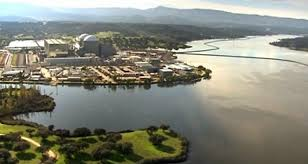
\includegraphics[width=0.47\textwidth]{2Introduction/ArrocampoDam.jpeg}}
  \subfloat[Tajus river along Spain and Portugal]{
   \label{fig:TajusRiver}
    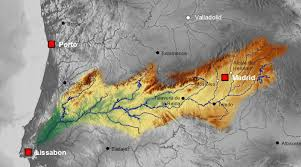
\includegraphics[width=0.53\textwidth]{2Introduction/RioTajo.jpeg}}
 \caption{Arrocampo dam, Almaraz NPP and Tajus river}
 \label{fig:Arrocampo}
\end{figure}

As it has been said, the \textit{Tritium} collaboration is a international group consisting of a consortium of 6 different southwestern european institution of 3 different countries: The University of Aveiro, in Portugal, The University of Bordeaux and the National Center for Scientific Research, CNRS  (Section Aquitaine-Limousin), in France and the University of Extremadura, \textit{Junta de Extremadura} and University of Valencia, in Spain.

FOTOOS PERSONAS TRITIUM

Each institution has focused in the development of a different part of all this project:
\begin{itemize}
\item{} First, the Extremadura group has developed and installed the ultrapure water system with wich water with very low conductivity, $\sigma \approx 10~\mu\sievert/\cm$ (two orders less than sample before the cleaning process, $1000~\mu\sievert/\cm$) is achieved. This clean process is very important for two reasons. On the one hand, it is important for maintaining our detector very clean, which is a critical point. On the other hand, it's important because with this process the natural background is reduced since several natural radiactive isotopes that there are in this water (except tritium) are removed such as $\ce{^{222}Rn}$, $\ce{^{40}K}$ or $\ce{^{137}Cs}$. This system will be explained in section \ref{sec:UltraPureWaterSystem}.

\item{} Second, french group has develop the pasive shielding where our detector will work inside. It is based in ultra radiopure lead with very low intrinsic activity. The objective of this pasive shielding is to reduce the external natural background that affect to our system. Obviously, this shielding doesn't have to affect to the measurement of our system, this is why radiopure elements with very low intrinsic activity are used (lead in the TRITIUM case). This shielding will be explained in section \ref{subsec:SetUpPassiveShield}.

\item{} Third, The Portugal and Spain people has collaborated for designing, developing and building four different prototypes of tritium detector and active vetos for removing cosmic events. These prototypes and vetos will be explained in the chapter \ref{chap:Prototypes} and section \ref{subsec:SetUpActiveShield} respectively.

\item{} Lastly, The Portugal and Spanish people has also developed the simulations about this system. The environment chosen to develop these simulations is GEANT4, which is a simulation package. It consists in a extensive C++ library with which the geometry of our detector, the physical processes which happen there, etc. can be designed. This simulation will be explained in the chapter \ref{chap:Simulations}.

\end{itemize}

The tritium level to be mesured follow the ALARA principle (As Low As Possible Achievable) and to get it there are important characteristics which our tritium detector must have:

\begin{itemize}

\item{} \textit{Compact}. This is important because in the place where this detector will be installed the useful space to be used is finite.

\item{} \textit{Thin active volume and large active area}. On the one hand, it have to be taken into account that, as it has been shown in Table \ref{tab:MeanFreePathTritium} of the section \ref{sec:TritiumProperties}, the mean free path of the $\beta$ particle of tritium decay is very low so thin active volumes are needed. In the practice, Active thickness beyond the mean free path of the tritium will only contribute to the background. On the other hand, as it has been checked in section \ref{sec:StateOfTheArt} the efficiency of this type of detector scales with the active area so it is needed to design our detector with the largest possible active area.

\item{} \textit{High sensitivity to tritium}. It has to be kept in mind that the tritium activities that will be measured are very low so it is needed to reduce as much as possible the non-detected tritium events.

\item{} \textit{High specificity to tritium}. The detector has to be able to distinguish the tritium signal of the signal of other radiactive elements which can be present in the initial sample.

\item{} \textit{Quasi-real time response}. It is important that our sistem can work in quasi-real time in order to detect any problem as fast as possible. 

\item{} \textit{Rugged system}. Finally, It has to be take into account that the objective will be installing an automatical system which will work during a lot of years without specialized people so it is needed that our monitor are rugged. 

\end{itemize}

In order to get the measurement in quasi-real time it is needed to work \textit{in situ}, that's, in the same place that the sample is taken. Working \textit{in situ} has some benefits for the detector such as faster and cheaper maintenance since the sampling process, chain of custody, etc. are eliminated, more frequent measurements and safer monitor since the personal exposure dose is reduced, changes in activity levels can be detected quickly and possible errors due to specialized personnel are eliminated.


%In order to get the measurement in quasi-real time it is needed to work \textit{in situ}, that's, in the same place that the sample is taken. Working \textit{in situ} has some benefits:

%\begin{itemize}
%\item{} a faster monitor because we eliminates the process of taking the sample, the chain-of-custody until this sample arrive to this laboratory and the complexity which involve these tasks. 

%\item{} a better monitor since if we can work \textit{in site}, our measurements can be more frequent hence we will can identify cahnges in the activity earlier.

%\item{} a cheaper monitor because we have not only the material costs attached to the sample collection, chain-of-custody of this sample, shipping of this sample to the laboratory, etc. but we have also eliminated the costs attached to the specialized staff who are involving in these tasks. Our detector will only need frequent calibrations each time in order to ensure its correct operation.

%\item{} a safer monitor since the personal exposure dose is reduced and the changes in activity are detected fastly. On top of that we remove the possibles mistakes which can be done by specialized staff.

%\end{itemize} 